% 230V Relæ

Relæet er implementeret som beskrevet i designdelen. Figur \ref{lab:Relay_inside} viser relæet som det er implementeret. Relæet er indbygget i en lukket kasse med transparent låg. 
Veroboard er benyttet som sokkel for relæet. Installationsledning er benyttet til 230V spændingen 0,75 kvadrat.
Den lyseblå leder er nul og den sorte leder er 230V fasen 
Jord/beskyttelseslederen er den gul/grønne, denne går direkte fra indgang (apparatstik) til udgang (230V stikkontakt). 
  


\begin{figure}[htb]
\centering
{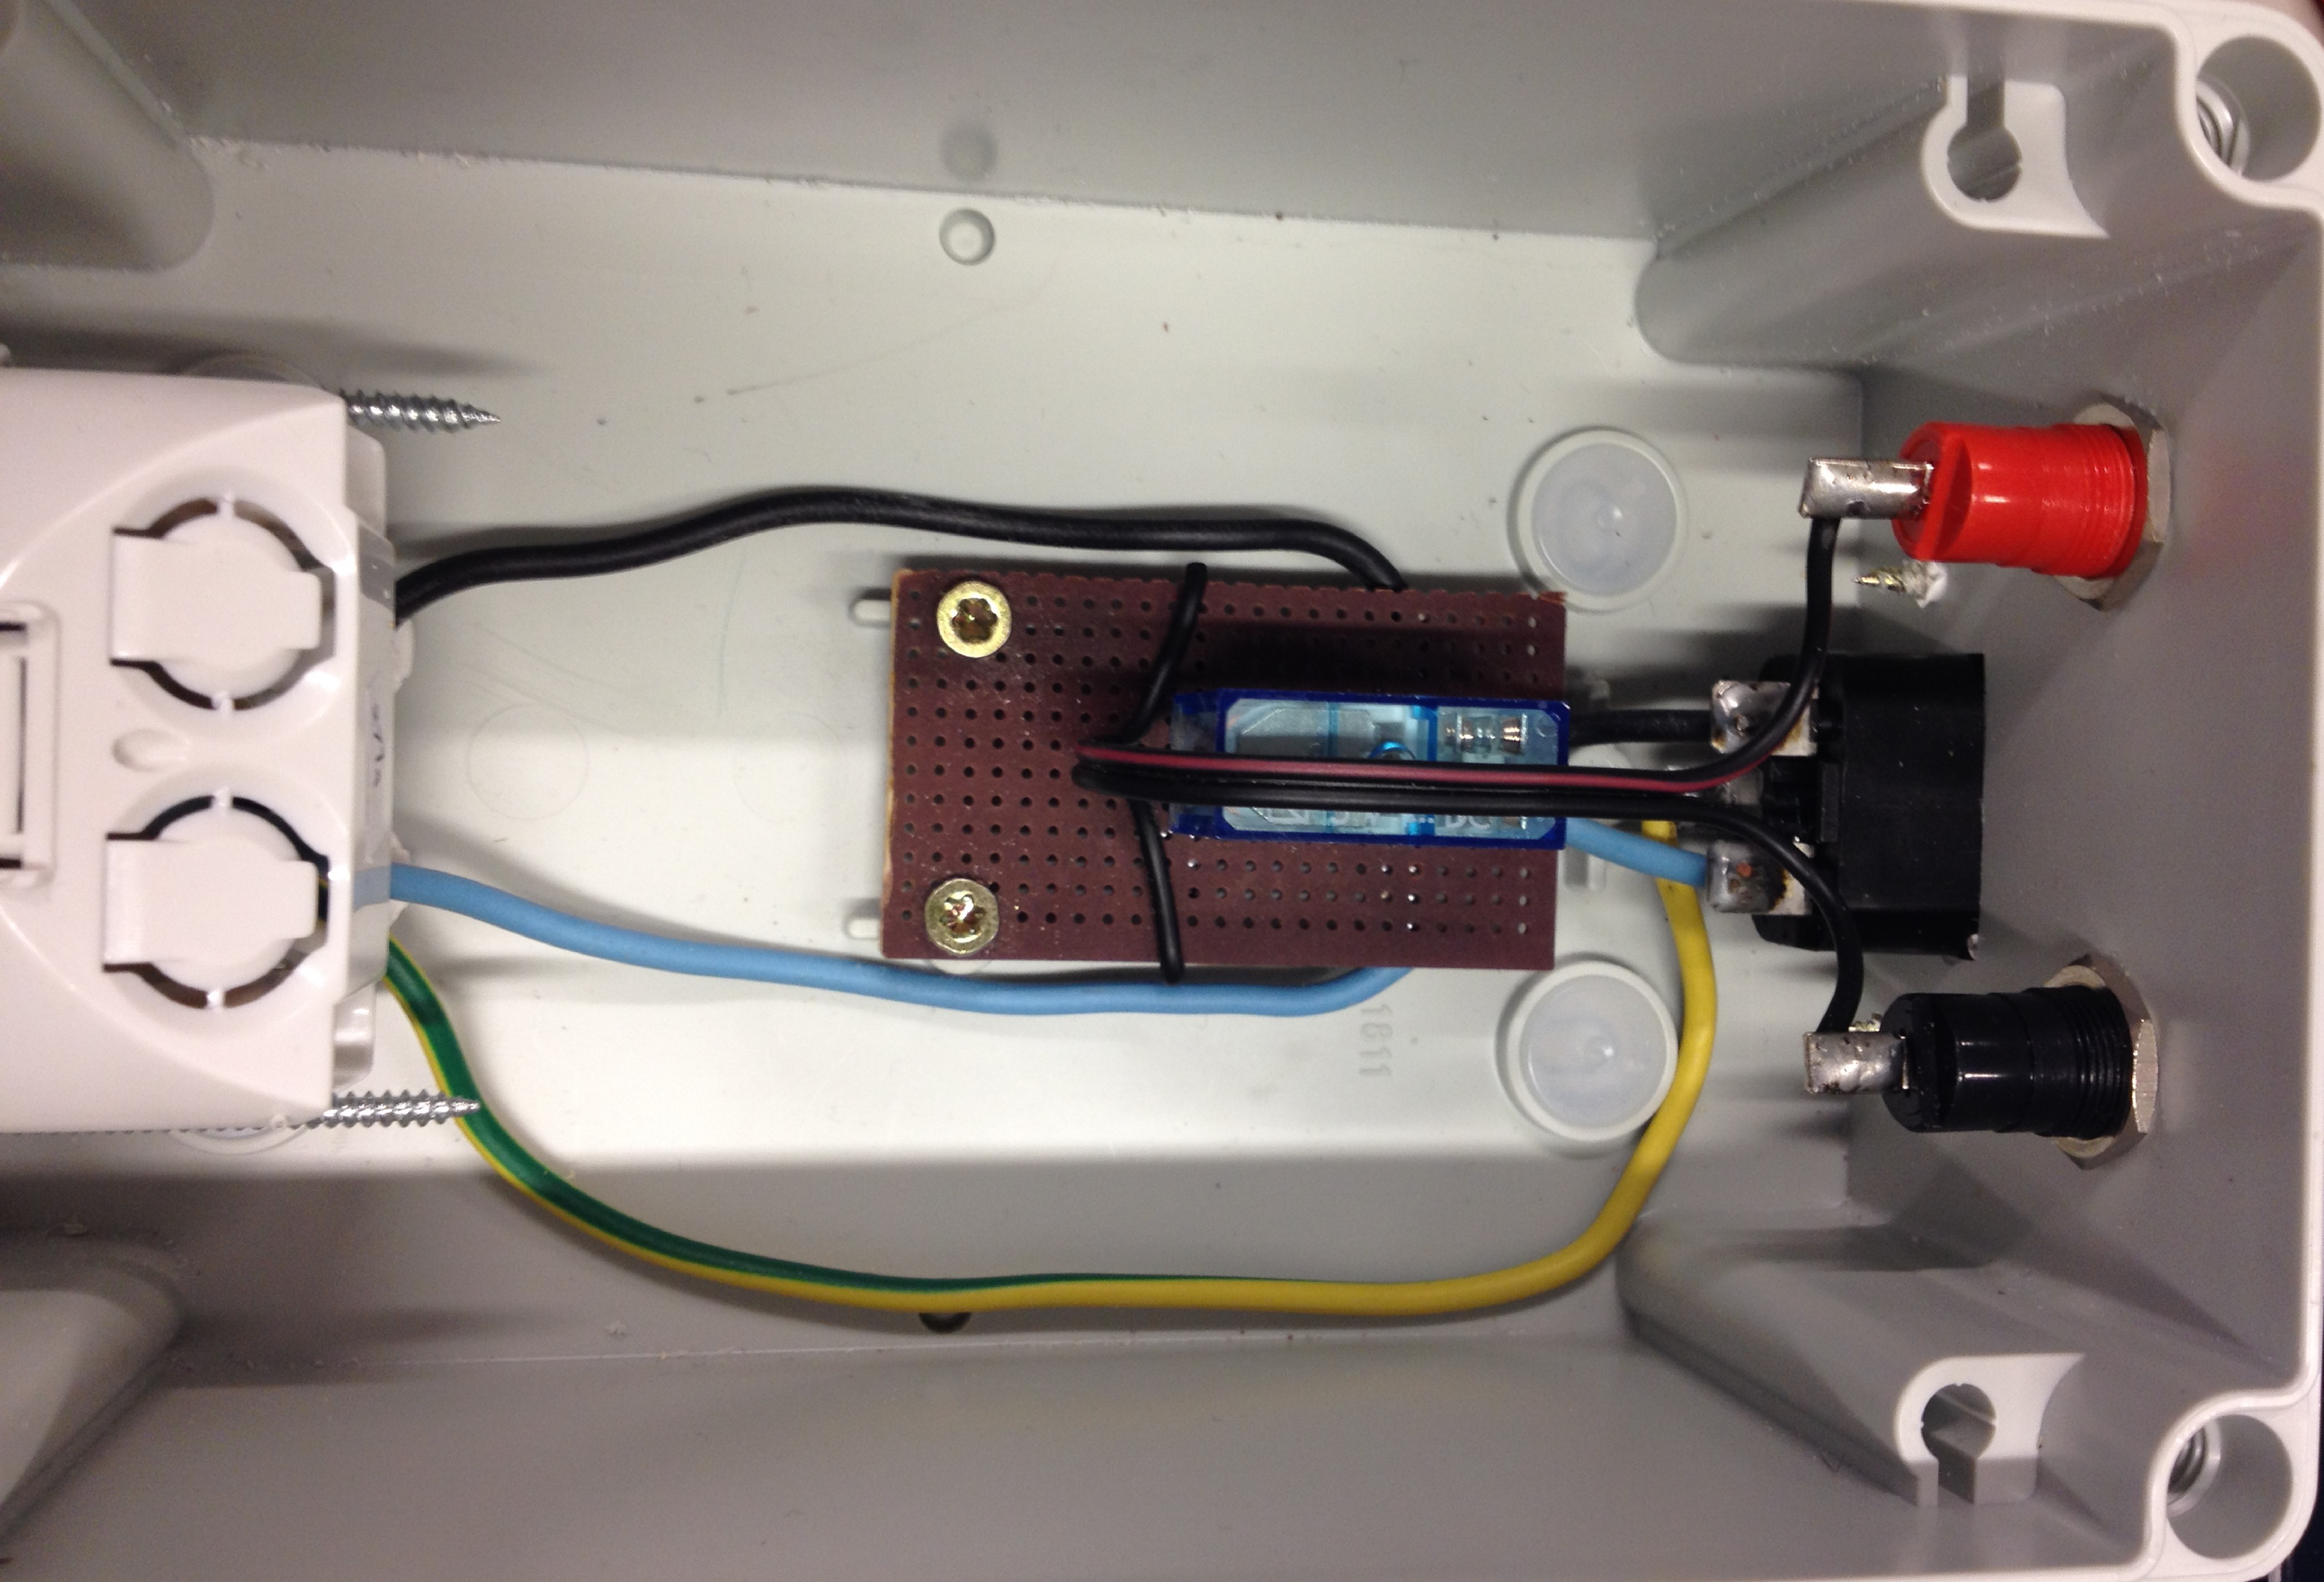
\includegraphics[width=0.60\textwidth]{filer/implementering/relay_inside}}
\caption{Relæet uden påmonteret låg}
\label{lab:Relay_inside}
\end{figure}

Figur \ref{lab:Relay_connection} viser relæet fra begge ender. Veste side viser indgangen, som består af ét 230V apparatstik og 2 bananstik. Apparatstikket tilsluttes en stikkontakt som er tændt. Bananstikkene tilsluttes tilslutningsprintet. Højre side viser 230V stikkontakten som tændes/slukkes af relæet. Vandpumpen tilsluttes denne stikkontakt.

\begin{figure}[htb]
\centering
{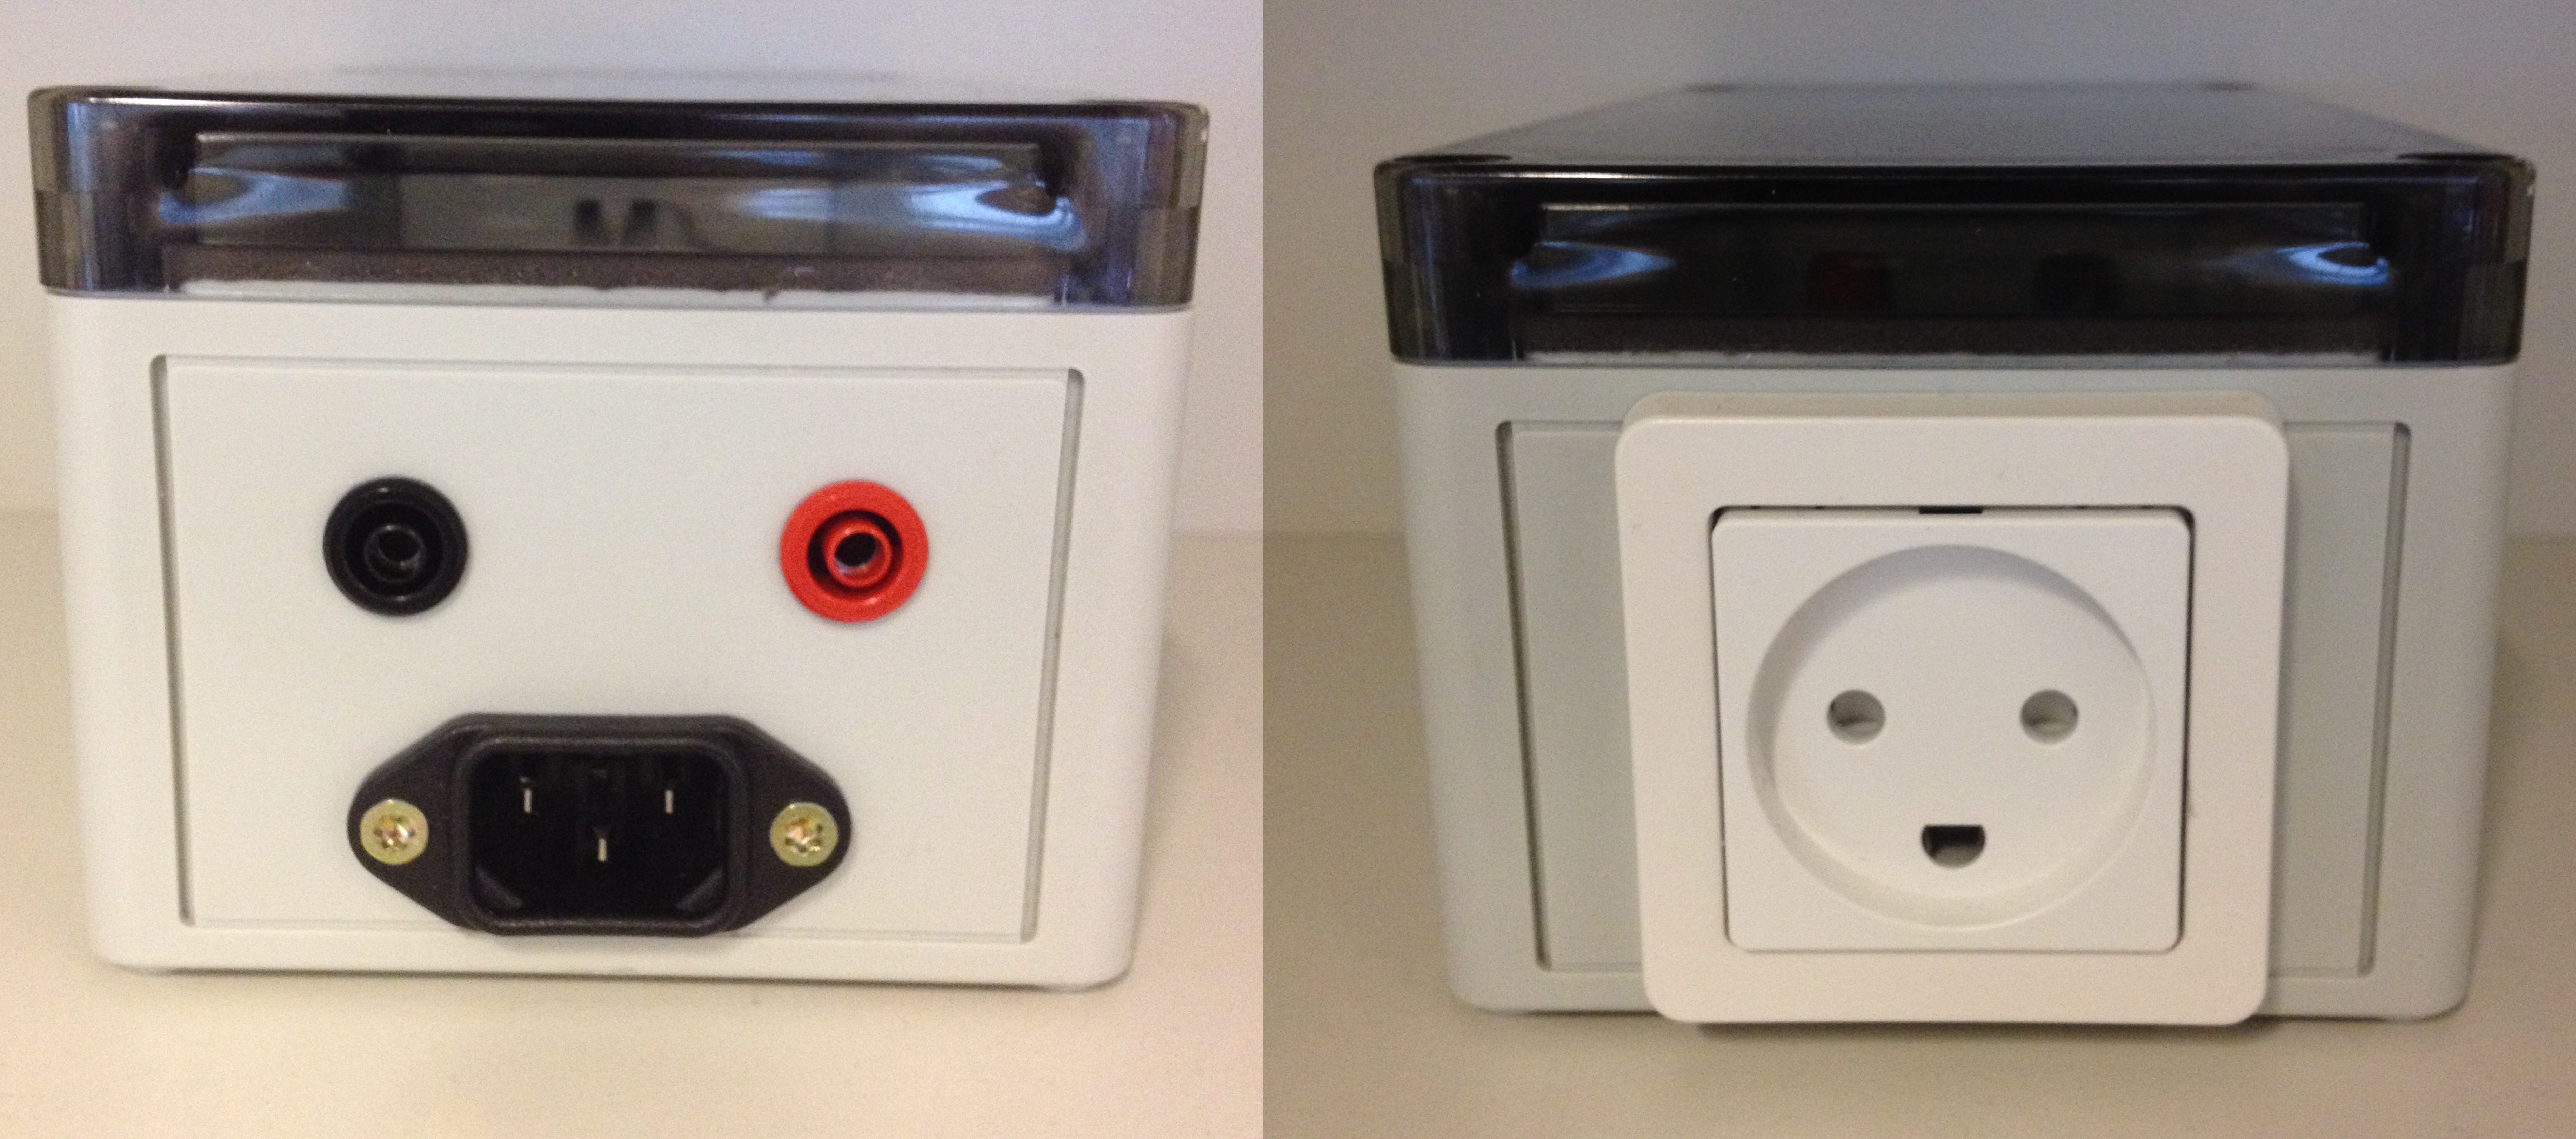
\includegraphics[width=0.80\textwidth]{filer/implementering/relay_connection}}
\caption{Relæet set fra begge ender.}
\label{lab:Relay_connection}
\end{figure}

Relæet er godkendt af Torben Lund Jensen fra værkstedet på IHA.